% Copyright 2004 by Till Tantau <tantau@users.sourceforge.net>.
%
% In principle, this file can be redistributed and/or modified under
% the terms of the GNU Public License, version 2.
%
% However, this file is supposed to be a template to be modified
% for your own needs. For this reason, if you use this file as a
% template and not specifically distribute it as part of a another
% package/program, I grant the extra permission to freely copy and
% modify this file as you see fit and even to delete this copyright
% notice. 

\documentclass{beamer}

% There are many different themes available for Beamer. A comprehensive
% list with examples is given here:
% http://deic.uab.es/~iblanes/beamer_gallery/index_by_theme.html
% You can uncomment the themes below if you would like to use a different
% one:
%\usetheme{AnnArbor}
%\usetheme{Antibes}
%\usetheme{Bergen}
%\usetheme{Berkeley}
%\usetheme{Berlin}
%\usetheme{Boadilla}
%\usetheme{boxes}
%\usetheme{CambridgeUS}
%\usetheme{Copenhagen}
%\usetheme{Darmstadt}
%\usetheme{default}
%\usetheme{Frankfurt}
%\usetheme{Goettingen}
%\usetheme{Hannover}
%\usetheme{Ilmenau}
%\usetheme{JuanLesPins}
%\usetheme{Luebeck}
\usetheme{Madrid}
%\usetheme{Malmoe}
%\usetheme{Marburg}
%\usetheme{Montpellier}
%\usetheme{PaloAlto}
%\usetheme{Pittsburgh}
%\usetheme{Rochester}
%\usetheme{Singapore}
%\usetheme{Szeged}
%\usetheme{Warsaw}

\usepackage{kotex}
\usepackage{braket}
\usepackage{array}
\usepackage{calc}
\usepackage{datetime}

\usepackage{listings}
\usepackage{dsfont}


\title{Lecture 2 : 수식의 파싱/벡터와 행렬}

% A subtitle is optional and this may be deleted
\subtitle{Fastcampus Math Camp}

\author{신승우}
% - Give the names in the same order as the appear in the paper.
% - Use the \inst{?} command only if the authors have different
%   affiliation.

% \institute[Universities of Somewhere and Elsewhere] % (optional, but mostly needed)
% {
  % \inst{1}%
  % Department of Computer Science\\
  % University of Somewhere
  % \and
  % \inst{2}%
  % Department of Theoretical Philosophy\\
  % University of Elsewhere}
% - Use the \inst command only if there are several affiliations.
% - Keep it simple, no one is interested in your street address.

% - Either use conference name or its abbreviation.
% - Not really informative to the audience, more for people (including
%   yourself) who are reading the slides online

\subject{Theoretical Computer Science}

% This is only inserted into the PDF information catalog. Can be left
% out. 

% If you have a file called "university-logo-filename.xxx", where xxx
% is a graphic format that can be processed by latex or pdflatex,
% resp., then you can add a logo as follows:

% \pgfdeclareimage[height=0.5cm]{university-logo}{university-logo-filename}
% \logo{\pgfuseimage{university-logo}}

% Delete this, if you do not want the table of contents to pop up at
% the beginning of each subsection:


\AtBeginSection[]
{
  \begin{frame}<beamer>{Outline}
    \tableofcontents[currentsection,hideallsubsections]
  \end{frame}
}

% Let's get started
\begin{document}

\begin{frame}
  \titlepage
\end{frame}

\begin{frame}{Outline}
  \tableofcontents[hideallsubsections]
  % You might wish to add the option [pausesections]
\end{frame}

% Section and subsections will appear in the presentation overview
% and table of contents.


\begin{frame}{수업 목표} 
\begin{itemize} 
\item 수식 파싱
\item 벡터와 행렬의 연산 구현 
\item 벡터의 선형독립 이해 
\end{itemize}
\end{frame}

\section{수식의 파싱} 

\subsection{파싱} 

\begin{frame}{What is Parsing?} 
\begin{block}{Parsing} 
특정 형식에 맞는 문자열을 원하는 데이터구조 형태로 만드는 것
\end{block}
\begin{itemize} 
\item \textbf{특정 형식}에 맞는 문자열 : Formal Grammar 
\item \textbf{원하는 데이터구조} : Abstract Syntax Tree(AST)
\end{itemize}
\end{frame}

% use for later slides on special lectures 
% \begin{frame}{Formal Grammar} 
% \begin{block}{Formal Grammar} 
% 형식 문법은 $N, T, P, S$의 4-tuple을 뜻하며, 각각은 다음과 같다.
% \end{block}
% \begin{itemize}
% \item N : Nonterminal Symbol 
% \item T : Terminal Symbol 
% \item P : production rules 
% \item S : Starting Symbol 
% \end{itemize}
% \end{frame}


% \begin{frame}{Formal Grammar} 
 
% 이 때, 각각은 다음의 조건을 만족해야 한다. 
% \begin{itemize}
% \item $N \cup T = \phi$
% \item $S \in N$
% \item P의 원소들은 $(N \cup T)*N(N \cup T)* -> (N \cup T)*$ 의 꼴. 
% \end{itemize}
% \end{frame}


\begin{frame}{수식의 Grammar} 
수식의 grammar를 살펴보면 다음과 같다. \\
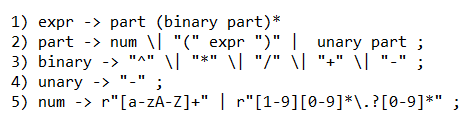
\includegraphics[width=10cm,keepaspectratio]{grammar}

1)에서 (binary part)*는 binary part의 유한한 반복을 뜻한다. 0번 반복하더라도 상관없다. 

\end{frame}

\begin{frame}{Syntax Check using Grammar}
위 문법에 기반하여 $x*(y+z)$ 가 수식의 문법에 맞는 문장인지 알아보자. 

\begin{table}[]
\centering
\caption{$x*(y+z)$ 체크}
\label{my-label}
\begin{tabular}{|l|l|l|}
\hline
current string & rule & result \\ \hline
x*(y+z)&1    & is x part?, is * binary?, is (y+z) part?      \\ \hline
x &  2, 3 & x is num! / num is part!      \\ \hline
*& 3    & * is binary!      \\ \hline
(y+z)& 3    &  is y+z expr?      \\ \hline
y, z& same to x    &   y,z is num! / num is part!   \\ \hline
+ & 3    &  + is binary!     \\ \hline
\end{tabular}
\end{table}

\end{frame}

\begin{frame}{Syntax Check using Grammar} 
이번에는 $x*(y+$ 가 수식의 문법에 맞는 문장인지 알아보자. 

\begin{table}[]
\centering
\caption{$x*(y+$ 체크}
\label{my-label}
\begin{tabular}{|l|l|l|}
\hline
current string & rule & result \\ \hline
x*(y+ & 1    & is x part?, is * binary?, is (y+ part?      \\ \hline
x &  2, 3 & x is num! / num is part!      \\ \hline
*& 3    & * is binary!      \\ \hline
(y+& 3    &  is y+ expr?      \\ \hline
y & same to x    &   y is num! / num is part!   \\ \hline
+ & 3    &  + is binary!     \\ \hline
eos &  None  &  expected part, return eos : \textbf{SyntaxError}     \\ \hline
\end{tabular}
\end{table}
이처럼, 위 문법에서의 규칙들을 순차적으로 적용하는 것으로 특정 문자열이 그 문법에 맞게 작성되었는지를 알 수 있다. 이럴 때 그 특정 문자열은 그 문법에 의해서 생성되었다고 한다. 

\end{frame}


\subsection{Abstract Syntax Tree} 

\begin{frame}{Abstract Syntax Tree} 

구문의 문법 구조를 반영하여 트리 형태로 나타낸 것을 abstract syntax tree라고 한다. 예를 들어서, 위 $x*(y+z)$의 경우 다음과 같은 트리로 생각할 수 있다. 

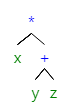
\includegraphics[height=5cm,keepaspectratio]{ast}

이때까지 문법과 그 문법을 이용하여 파싱한 결과물이 무엇인지 간략하게 살펴보았다. 이제 본격적으로 어떤 식으로 구현하는지 살펴 보고자 한다. 

\end{frame}


\subsection{Recursive Descent Algorithm}

\begin{frame}{Parser Structure} 

먼저, 일반적인 파서의 구조를 살펴보자. 일반적으로 파서는 두 가지 함수로 이루어져 있다. 

\begin{itemize} 
\item tokenizer : string to tokens
\item parser : tokens to AST
\end{itemize}

여기서, token이란 최소한의 의미를 가지는 문자열을 말한다. 문법에서 "으로 둘러싸인 문자열이나 그 문자열이 나타내는 정규표현식과 일치하는 문자열을 뜻한다. 

\end{frame}

\begin{frame}{Implementing Tokenizer} 

Tokenizer의 경우, 다음의 과정을 통해서 만들 수 있다. 

\begin{itemize} 
\item 문법에서 token의 패턴을 추출한다. 
\item input string에 대해서, input string == '''' 가 될 때까지 
\begin{itemize}
\item 각 패턴에 대해서 check re.match(pattern, input string)
\item 만약 맞으면 input string에서 pattern과 일치하는 부분을 yield
\item 일치하는 부분을 제외한 나머지를 input string으로 업데이트
\item 만약 모든 패턴에 대해서 맞지 않으면 SyntaxError 리턴
\end{itemize}
\end{itemize}
\end{frame}

\begin{frame}{Shunting-Yard Algorithm} 

이제 얻어진 token들을 이용하여 abstract syntax tree를 만드는 알고리즘을 생각해 보자. 먼저, 스택 2개를 생각한다. 

\begin{itemize} 
\item operand stack 
\item operation stack 
\end{itemize}

이 때, operation stack에서는 필요한 operand들이 파싱이 끝날 때까지 operation을 pop하지 않는다. 또한, operation들 중 더 우선순위가 높은 operation이 항상 스택의 위에 오도록 유지한다. 예를 들어서, operation stack에 /가 있을 때, +가 들어오기 전에 /를 pop하고 필요한 처치를 한다. 즉, 그 때 operand stack의 가장 위에 있는 token 2개를 pop\footnote{만약 operation이 unary라면 1개. operation에 맞는 갯수를 리턴하면 된다.}  하여 Tree('/', tok1, tok2) 형태로 만드는 것이다. 만약 그 때 operand stack에 2개의 token이 없다면 에러를 리턴한다. operator가 스택에서 pop될 때마다 tree가 하나씩 생성되며, 이를 다시 operand stack에 push한다.

파싱이 되는 예시 2개와, 되지 않는 예시 1개를 들어서 살펴보고 이를 구현해보겠다. 

\end{frame}

\begin{frame}{예시}
\begin{table}[]
\centering
\caption{$x*y+z$ 파싱 예제}
\label{my-label}
\begin{tabular}{|l|l|l|l|}
\hline
tokens & operand  & op  & action \\ \hline
x, *, y, +, z &     &  & operand.push(x)     \\ \hline
*, y, +, z &  x   &  & compare(*, None)     \\ \hline
, y, +, z &  x   & * & operation.push(*)    \\ \hline
y, +, z &  x   & * & operand.push(y)     \\ \hline
+, z &  y, x  & * & compare(*, +)     \\ \hline
+, z &  Tree(*, [x, y])   &  & operator.pop()     \\ \hline
z &  Tree(*, [x, y])   & + & operation.push(+)     \\ \hline
&  z, Tree(*, [x, y])   & + & operand.push(z)     \\ \hline
&  Tree(+, [z, Tree(*, [x, y])])   &  & operation.pop()     \\ \hline
\end{tabular}
\end{table}


\end{frame}



\begin{frame}{예시}

\begin{table}[]
\centering
\caption{$x*(y+z)$ 파싱 예제}
\label{my-label}
\begin{tabular}{|l|l|l|l|}
\hline
tokens & operand  & op  & action \\ \hline
x, *, (,  y, +, z, )&     &  & operand.push(x)     \\ \hline
*, (,  y, +, z, )&  x  &  & operation.push(*)     \\ \hline
(,  y, +, z, )&  x  & * & parse(find\_match(tokens, 0))     \\ \hline
 &  Tree(+, [y,z]) x  & * & operand.push(parse(..))     \\ \hline
 &  Tree(+, [y,z]) x  & * & operator.pop()     \\ \hline
 &  Tree(*, [Tree(+, [y,z]), x]  &  & operator.pop()     \\ \hline
\end{tabular}
\end{table}

여기서 find\_match 함수를 사용하는데, 이는 tokens에서 어떤 index의 괄호와 쌍을 이루는 괄호를 찾는 것이다. 이를 통해서 괄호 안의 식을 우선적으로 처리할 수 있다. 

\end{frame}


\begin{frame}{예시}

\begin{table}[]
\centering
\caption{$y+$ 파싱 예제}
\label{my-label}
\begin{tabular}{|l|l|l|l|}
\hline
tokens & operand  & op  & action \\ \hline
y, + &     &  & operand.push(y)     \\ \hline
 + &  y   &  & operator.push(+)     \\ \hline
 &  y   & + & operator.pop()     \\ \hline
 &  y   & + & operand.pop();operand.pop()     \\ \hline
 &  y   & + & raise SyntaxError     \\ \hline
\end{tabular}
\end{table}

\end{frame}


\begin{frame}{Implementing Parser} 

위에서 알고리즘의 개요를 살펴보았다. 이제 본 알고리즘을 구현해볼 것이다. 본격적인 구현 전에, 필요한 변수들과 함수들을 구현하자. 
\begin{itemize} 
\item precedence : operator들 간 우선순위를 저장한 변수
\item find\_match 함수 : 맞는 괄호 찾아주기 
\item compare 함수 : operator 간 우선순위 비교
\end{itemize}

이후, 스택 두 개를 만들어 위 알고리즘을 구현한다. 
\end{frame}

\begin{frame}{Implementing Parser : 실습/quiz}
 
실습은 skeleton/PyFormula.py 에서 tokenizer 함수와 parser 함수를 짜서 아래의 test들을 다 통과하면 됩니다. Tree의 형태가 다르더라도 같은 식을 만들면 맞는 걸로 인정합니다. 문법은 다음과 같습니다. 

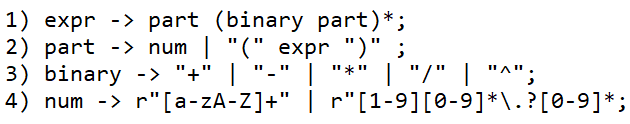
\includegraphics[width=10cm,keepaspectratio]{simplegrammar}

실습에서는 
\begin{itemize} 
\item operator 순서는 \textasciicircum, (*, /), (+, -) 순입니다. 
\item \textbf{unary는 고려하지 않습니다.}
\item tokenizer 함수는 token을 만드는 genertor나, list 형태로 리턴하면 됩니다. 
\item parser은 util.py에 있는 Tree의 인스턴스나 3-tuple 형태의 답을 리턴하면 됩니다. 예를 들어서 (1+2)*3 이라면, (* (+ 1 2) 3) 혹은 (* 3 (+ 1 2)) 형태로 출력하면 됩니다.
\end{itemize} 


\end{frame}

\begin{frame}{Implementing Parser}

30분 동안, 주어진 파일 내의 스켈레톤 코드와 주석의 힌트를 활용하여 짜 보시면 됩니다. 30분 안에 다 짜신다면, unary operator를 추가해 보세요. 

open problem이므로 굉장히 많은 방법이 가능합니다. 꼭 recursive descent를 쓰지 않아도 되며, 어떤 식으로던 테스트만 통과한다면 맞는 답안일 것입니다. 

짜신 후에 결과물을 principia\_12@kaist.ac.kr로 보내주시면 감사하겠습니다. 다 못 짜셔도 괜찮습니다. 
\end{frame}

\begin{frame}{Looking at Parser Implementation} 
이제 테스트를 다 통과하는 하나의 답을 보겠습니다. (절대 유일한 답이 아닙니다!) 
\end{frame} 

\begin{frame}{Further Topic : Automatic Parser Generation} 
위 파서 구현과 문법을 비교해 보자. 상당히 유사함을 알 수 있다. 이는 문법 문자열을 파싱하여 자동으로 그 문법에 맞는 파서를 작성할 수 있음을 시사한다. 이는 lex나 yacc 등의 라이브러리를 사용하여 자동으로 생성할 수 있다. 이에 대해서는 특강에서 자세히 다룰 예정이다. 
\end{frame}

\begin{frame}{Adding Unary Operator} 
아까의 문제에서는 Unary Operator가 빠져 있습니다. 이제 Unary Operator를 넣어 보겠습니다. 여기서는 unary operator의 우선순위를 최상위로 둡니다. 


앞으로 이런 식으로 지금 짜여진 파서에 다양한 기능을 조금씩 추가하여 수식을 확장할 것입니다. 일종의 수식 언어 인터프리터를 짠다고 생각하시면 될 것 같습니다. 
\end{frame}


\subsection{수식의 계산} 

\begin{frame}{Evaluation of AST} 

이제 파싱된 결과물을 이용하여 수식의 값을 계산하는 것은 직관적으로 이루어질 수 있다. \\

Tree(op, [arg1, arg2])

의 evaluation 결과는 \\

evaluation(arg1) op evaluation(arg2) \\

로 재귀적으로 구할 수 있기 때문이다. 여기서 evaluation의 결과물이 숫자일 경우, 아무런 문제가 없다. 하지만 만약 변수가 들어가 있다면 어떻게 될까? 
\end{frame}

\begin{frame}{PyFormula : Apply Variables} 

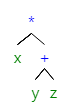
\includegraphics[height=5cm,keepaspectratio]{ast}

이 경우, x,y,z 3개의 input을 받는 함수로 생각할 수 있다. 따라서 본 수업에서는 ast를 함수로 만들어주는 일종의 wrapper를 구현할 것이다. 이를 PyFormula라 하고, 앞으로 쭉 사용될 것이다. 
\end{frame}

\begin{frame}{Implementing PyFormula} 
PyFormula는 다음의 operation들을 지원한다. 
\begin{itemize}
\item 사칙연산 
\item str()
\item \_\_call\_\_
\item \_calculate (staticmethod)
\item \_tree2str (staticmethod) : 너무 길어 수업중에 구현하지 않는다. 
\end{itemize}
그 외의 함수들은 차차 필요에 따라 구현해 나갈 것이다. 
\end{frame}




\subsection{Tensorflow Computational Graph} 

\begin{frame}{Computational Graph} 

이렇게 계산을 위해서 트리 형태로 만들 수도 있지만, 텐서플로우에서는 Computational Graph라는 다른 형태의 계산 형식을 제공한다. 
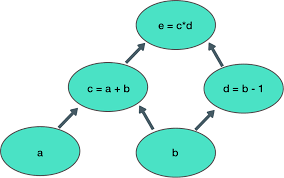
\includegraphics[height=5cm,keepaspectratio]{compgraph}

이는 사실 트리의 노드들을 vertex로 만들고, 조상-자손 관계를 edge로 만들면 쉽게 변형할 수 있다. 따라서 본질적으로 똑같은 구조이지만, 그래프 형태가 계산에서 이점이 있다. 일종의 memoization을 제공하기 때문이다. 
\end{frame}


\section{벡터} 

\subsection{motivation}

\begin{frame}{Motivation} 

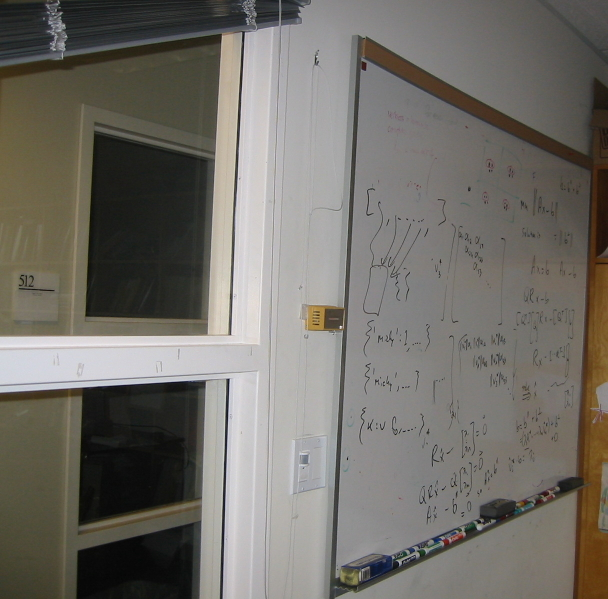
\includegraphics[height=5cm,keepaspectratio]{board}

위 사진에서, 화이트보드 위에 쓰인 글을 정면에서 바라보는 사진을 얻을 수 있을까? 

\end{frame}

\begin{frame}{Motivation} 
기지국에서 각 고객들의 핸드폰으로 신호를 보낼 때, 각 핸드폰이 수신하는 신호는 다 같을 것이다. 이 때, 각 고객은 어떻게 본인에게 맞는 신호를 수신하는가? 

놀랍게도 이 두 문제는 사실상 같은 수학적 구조를 사용한다. 
\end{frame}


\subsection{벡터의 정의} 

\begin{frame}{벡터의 정의} 
\begin{itemize} 
\item 기하학적 직관 : 화살표 
\item 실용적 정의 : $PyFormula^n$
\item 추상적 정의 : vector space axioms
\end{itemize}
\end{frame}

\begin{frame}{직교좌표계} 
\begin{block}{좌표계}
좌표란 공간\footnote{더 엄밀하게는 유클리드 공간} 내에서 한 점을 유일하게 결정하기 위해서 필요한 숫자들을 말하며, 공간 전체를 나타내기 위해서 필요한 좌표의 집합을 좌표계라 한다. 
\end{block}

예를 들어서, 1차원 공간(선)을 생각해 보자. 선 위에서의 한 점을 결정하기 위해서는 어떤 특정한 점에서의 거리만 있으면 충분\footnote{절대로 유일하다는 것이 아니다! 다른 방법으로도 나타낼 수 있지만, 이 방법으로도 모든 점을 나타낼 수 있다는 뜻이다.}하다. 

\end{frame}
\begin{frame}{직교좌표계} 
2차원 공간이라면 아래와 같이 

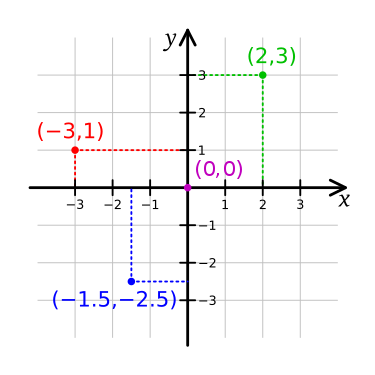
\includegraphics[height=5cm,keepaspectratio]{cartesian}

2개의 수직한 선에서의 거리를 이용하여 나타낼 수 있다. 이런 식으로 수직한 n개의 선에서의 거리로 좌표를 표현하는 것을 직교좌표계라고 한다. 
\end{frame}

\begin{frame}{좌표계에서 도형의 방정식} 
이제 우리는 좌표계를 이용하여 공간 내 모든 점에 좌표를 부여할 수 있다. 이제, 공간 내에서 특정 조건을 만족하는 점들의 집합을 도형이라고 부를 것이다. 예를 들어서, 2차원 공간에서의 (0,0)을 중심으로 하는 원은 다음의 조건을 만족하는 좌표에 대응되는 점들의 집합이다. 

$\{(x,y)|x^2+y^2<1\}$

보통 위와 같이 $\{(x,y)|f(x,y)<0\}$ 형태로 주어지며, 이 때 f를 도형의 방정식이라고 한다. 
\end{frame}


\begin{frame}{벡터의 기하학적 직관} 
% 그림 
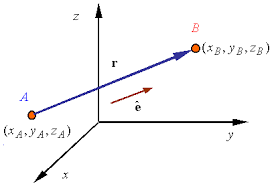
\includegraphics[height=5cm,keepaspectratio]{vec}

기하학적으로 벡터는 두 점 사이의 변위를 말한다. 

\end{frame}

\begin{frame}{벡터의 실용적 정의 } 

일반적으로 n-벡터는 숫자 n개로 정의된다. 하지만 여기서는 추후 벡터와 미적분, 함수의 결합을 위해서 다음과 같이 정의한다. 

\begin{block}{벡터} 
n-벡터란 숫자, 혹은 PyFormula n개의 순서쌍이다. $\vec{v}$와 같이 위에 화살표를 써서 표기한다. 
\end{block} 

벡터와 대응되는 개념으로 스칼라가 있다. 

\begin{block}{스칼라} 
스칼라는 1-벡터이다. 
\end{block}

이제 벡터의 연산을 정의해보자. 

\end{frame}

\subsection{벡터의 연산} 

\begin{frame}{벡터의 연산 : 더하기, 스칼라곱} 
두 벡터 v, u가 $\vec{v} = (v_i), \vec{u} = (u_i), i = 1,2, ..., n$ 이라고 할 때, 벡터의 덧셈/뺄셈과 스칼라곱은 다음과 같이 정의된다. 
\begin{itemize} 
\item $\vec{v} + \vec{u} = (v_i + u_i)$
\item $\vec{v} - \vec{u} = (v_i - u_i)$
\item $c\vec{v} = c*v_i $
\end{itemize}
0벡터는 $\vec{v} + \vec{0} = \vec{0} + \vec{v} = \vec{v}$ 인 벡터를 말한다. 
\end{frame}

\begin{frame}{벡터의 연산 : 기하학적 직관} 
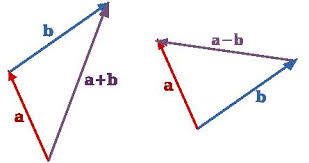
\includegraphics[height=5cm,keepaspectratio]{addition}
\end{frame}

\begin{frame}{직선/선분의 방정식} 


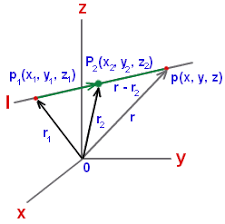
\includegraphics[height=5cm,keepaspectratio]{line}
\begin{block}{직선}
직선은 두 벡터 $\vec{r_1}, \vec{r_2}$가 주어졌을 때, 다음과 같은 집합을 말한다. $\{\vec{r}|\vec{r} = \vec{r_1} + \lambda (\vec{r_1} - \vec{r_2})\}$
\end{block} 

선분은 집합의 부분집합이다. 

\end{frame}

\begin{frame}{벡터의 연산 : 내적/크기} 
두 벡터 v, u가 $\vec{v} = (v_i), \vec{u} = (u_i), i = 1,2, ..., n$ 이라고 할 때, 벡터의 내적/크기와 orthogonality는 다음과 같이 정의된다. 

\begin{itemize} 
\item $ \vec{v} \bullet \vec{u} = \sum_{i}^{n} v_i * u_i $
\item $ |\vec{V}| = \sqrt{\vec{v} * \vec{v}} $ 
\item $ \vec{v} \bullet \vec{u} = 0 $이면 벡터 v,u가 orthogonal하다. 
\end{itemize}

위에서 볼 수 있듯이, 벡터의 크기는 내적을 이용하여 정의된다. 
\end{frame}

\begin{frame}{평면의 방정식} 
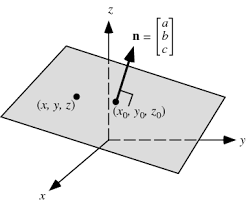
\includegraphics[height=5cm,keepaspectratio]{plane}
\begin{block}{평면}
평면은 벡터 $\vec{n}$이 주어졌을 때, 다음과 같은 집합을 말한다. $\{\vec{r}|\vec{n} \bullet \vec{r} = 0\}$
\end{block} 
이 때 $\vec{n}$을 법선 벡터라 한다. 
\end{frame}



\begin{frame}{hyperplane} 
n차원 공간에 대해서, n-1차원 hyperplane은 다음과 같이 정의된다. 
\begin{block}{hyperplane} 
hyperplane은 n-벡터 $\vec{n}$에 대하여 $\{\vec{r} | \vec{r} \bullet \vec{n} = 0\}$을 말한다. 
\end{block}

예를 들어서, 2차원 공간에서의 hyperplane은 1차원 선이며, 3차원 공간에서의 hyperplane은 평면이다. 
\end{frame}

\begin{frame}{선형 방정식과 그 계} 

\begin{block}{선형방정식}
선형방정식은 다음과 같은 식을 말한다. $\sum^{n}_{i=1} a_i x_i = y$ 

위 내적의 정의를 이용하면, 다음과 같이 쓸 수도 있다. $ \vec{a} \bullet \vec{x} = y$
\end{block}

\begin{block}{선형방정식의 계와 그 해 }
선형방정식의 모음을 말하며, 보통 다음과 같이 쓴다. $\sum^{n}_{i=1} a_ij x_i = y_j, j=1,2, ... ,m $ 

위 내적의 정의를 이용하면, 다음과 같이 쓸 수도 있다. $ \vec{a_j} \bullet \vec{x} = y_j$

선형 방정식의 해는 선형방정식의 계를 만족하는 $\vec{x}$의 집합이다.
\end{block}

\end{frame}

\begin{frame}{벡터의 연산 : 외적 } 

두 벡터 v, u가 $\vec{v} = \{v_1, v_2, v_3\}, \vec{u} = \{u_1, u_2, u_3\}$일 때, 두 벡터의 외적은 다음과 같이 정의된다. 
\begin{itemize} 
\item $\vec{v} \times \vec{u} = (v_2u_3 - v_3u_2, v_3u_1 - v_1u_3, v_1u_2 - v_2u_1) $
\end{itemize}

외적은 3차원 벡터에서만 적용되며, 교환법칙이 성립하지 않는다. 외적에 대해서는 다음의 법칙들이 성립한다. 

\begin{itemize} 
\item $\vec{v} \times \vec{u} = - \vec{u} \times \vec{v} $
\item $\vec{v} \bullet (\vec{v} \times \vec{u}) = 0 $
\item $\vec{u} \bullet (\vec{v} \times \vec{u}) = 0 $
\end{itemize}
\end{frame}


\begin{frame}{평면의 방정식 다시보기} 
평면을 다음과 같이 정의할 수도 있다. 즉, 두 벡터 $\vec{v}, \vec{u}$에 대해서 $\vec{v}$가 $\vec{u}$의 스칼라곱이 아니라면, $\{\vec{r}|\vec{r} \bullet (\vec{v} \times \vec{u}) = 0$ 도 평면의 방정식이 된다. 
\end{frame}

\subsection{선형결합과 벡터공간} 


\begin{frame}{Motivation} 

3차원 공간에서 어떤 평면 위의 점을 나타내는 좌표계를 찾을 수 있을까? 이 때, 

\begin{itemize} 
\item 항상 찾을 수 있을까? 
\item 그 좌표계가 유일할까? 
\item 유일하지 않다면, 좌표계끼리의 변환이 가능한가? 어떻게 가능할까? 
\end{itemize}

\end{frame}

\begin{frame}{몇 가지 개념들} 
\begin{block}{선형결합} 
벡터들 $\vec{v_i}, i=1,2,...,n$에 대하여 $\vec{v_i}$들의 선형결합은 $\sum c_i \vec{v_i}$이다. 
\end{block}

\begin{block}{span} 
벡터들 $\vec{v_i}, i=1,2,...,n$에 대하여 $span(\vec{v_i})$는 $\vec{v_i}$ 들의 선형결합으로 나타낼 수 있는 벡터들의 집합이다. 
\end{block}
\end{frame}



\begin{frame}{좌표계와 Span에 대한 직관적 접근 } 
\begin{block}{좌표계}
좌표란 \textbf{공간} 내에서 한 점을 \textbf{유일하게} 결정하기 위해서 필요한 \textbf{유한한 갯수의 숫자들}을 말하며, 공간 전체를 나타내기 위해서 필요한 좌표의 집합을 좌표계라 한다. 
\end{block}

\begin{block}{span} 
벡터들 $\vec{v_i}, i=1,2,...,n$에 대하여 $span(\vec{v_i})$는 $\vec{v_i}$ 들의 선형결합($c_i$)으로 나타낼 수 있는 \textbf{벡터들의 집합}이다. 
\end{block}
\end{frame}


\begin{frame}{좌표계와 Span에 대한 직관적 접근 } 
선형결합을 통해서 어떤 벡터의 집합이 span하는 공간 내의 한 점을 $c_i$들을 이용하여 나타낼 수 있다. 이제, 문제는 2가지이다. 

\begin{itemize} 
\item 한 점을 유일하게 표현할 수 있는가?
\item 우리가 나타내고 싶어하는 공간을 span하면서 유일표현을 가능하게 하는  벡터 집합이 존재하는가?
\end{itemize}

이를 생각하기 위해서 몇 가지 개념들을 더 도입하겠다. 

\end{frame}


\begin{frame}{선형독립/종속} 
\begin{block}{선형독립/종속}
이 때 $\sum c_i \vec{v_i} = 0$인 $c_i$가 존재하면 $\vec{v_i}$들을 선형종속이라고 하고, 그러한 $c_i$가 $c_i=0$ 외에 존재하지 않으면 선형독립이라고 한다. 이 때 $\vec{v_i}$는 0벡터가 아니다. 
\end{block}
이 때, 
\begin{itemize} 
\item 선형종속인 벡터들 $\vec{v_i}$에 대해서, 그 중 하나의 벡터는 다른 벡터들의 선형결합으로 표현가능하며 역도 성립한다. 
\item 선형독립인 벡터들 $\vec{v_i}$에 대해서 2.1) $\sum c_i\vec{v_i} = \sum d_i\vec{v_i}$인 것과 2.2) $c_i = d_i$ 인 것은 동치이다. 
\item 선형독립인 벡터 집합 $\vec{v_i}$에서, $span(\vec{v_i}, i = 1, 2, ... , n-1) \subset span(\vec{v_i}, i = 1, 2, ... , n) $ 이다.  
\item 선형종속인 벡터 집합 $\vec{v_i}$에서, 선형 독립인 부분집합 $\vec{u_i}$를 찾을 수 있다. 
\item 모든 벡터간 서로 내적이 0인 벡터의 집합은 선형독립이다. 
\end{itemize}
\end{frame}

\begin{frame}{Proof for 1)} 

선형종속이면 $\sum c_i \vec{v_i} = 0$가 성립해야 하는데, 이는 곧 다음을 의미한다. 
\begin{eqnarray} 
\sum^n_{i=1} c_i \vec{v_i} & = & c_1 \vec{v_1} + \sum^n_{i=2} c_i \vec{v_i} \\
c_1 \vec{v_1} &=& - \sum^n_{i=2} c_i \vec{v_i}\\
\vec{v_1} &=& \sum^n_{i=2} -\frac{c_i}{c_1} \vec{v_i}
\end{eqnarray}
따라서, $\vec{v_1}$을 $\vec{v_2}, \vec{v_3}, ... \vec{v_n}$ 의 선형결합을 이용하여 나타내었으므로 참이다. 
반대로, $\vec{v_1} = \sum^n_{i=2} c_i \vec{v_i}$로 나타낼 수 있으면, $c_1=-1$이라 하면 $\sum c_i \vec{v_i} = 0$가 성립하므로 선형종속이므로 역도 성립한다. 

\end{frame}

\begin{frame}{Proof for 2.1) = 2.2)}

2.2)이면 2.1)임은 자명하다. 
2.1)이면 2.2)임을 보이기 위해서 귀류법을 사용하자. $\sum c_i\vec{v_i} = \sum d_i\vec{v_i}$이므로  $\sum (c_i-  d_i) \vec{v_i} = 0$이다. 선형독립의 정의에 따라서, $c_i - d_i=0$ 이므로 2.2)가 성립한다. 

\end{frame}

\begin{frame}{Proof for 3)} 
1)에 의해서 따라 $S = span(\vec{v_i}, i = 1, 2, ... , n-1)$에서는 $\vec{v_n}$을 $\vec{v_i}, i = 1, 2, ... , n-1$의 선형결합을 이용하여 나타낼 수 없다. 따라서 적어도 $\vec{v_n}$은 S의 원소가 아니다. 또한, $P = span(\vec{v_i}, i = 1, 2, ... , n)$은 적어도 S의 모든 원소를 포함하는데, 이는 $c_n=0$인 선형결합을 생각하면 자명하다. 따라서 S는 P의 진부분집합이다. 
\end{frame}

\begin{frame}{Proof for 4)} 
0벡터가 아닌 벡터 하나의 집합은 선형독립이다. 따라서 언제나 존재한다. 
\end{frame}

\begin{frame}{Proof for 5)} 
어떤 벡터집합 $\vec{v_i}$에 대해서, 임의의 다른 두 원소 $\vec{v_i}, \vec{v_j}$의 내적이 0이라고 하면 다음이 성립한다. 

$\forall j, \vec{v_j} \bullet \sum c_i \vec{v_i} = c_j |\vec{v_j}|^2$ 

따라서 $\sum c_i \vec{v_i} = 0$이기 위해서는 $\forall j, c_j=0$이여야 하므로, 선형독립이다. 
\end{frame}

\begin{frame}{Back to the question}

\begin{itemize} 
\item 한 점을 유일하게 표현할 수 있는가? : 선형독립인 벡터 집합으로 span되면 그렇다! (by 2))
\item 우리가 나타내고 싶어하는 공간을 span하면서 유일표현을 가능하게 하는 벡터 집합이 존재하는가? : 그렇다! (by 3), 4))
\end{itemize}

두 번째에 대해서 조금 더 설명하겠다. 먼저, 우리가 나타내고 싶어하는 공간에 있는 모든 벡터의 집합을 생각한다. 그 다음 유한한 subset을 고른다. 그 subset이 \textbf{전체 공간을 span}할 경우, \textbf{subset이 선형 독립}이 될 때까지 원소를 하나씩 제거한다. 만약 span하지 못할 경우, span할 수 있을 때까지 subset의 원소가 아닌 벡터를 골라서 추가한다. 이 과정을 반복하면, span이 우리가 원하는 공간이 되는 부분집합을 찾을 수 있으며, 이 부분집합이 선형독립이게 만들 수 있다. 다음 단락에서 이를 조금 더 정확하게 정의해 보겠다. 
\end{frame}

\subsection{기저의 정의} 

\begin{frame}{subspace의 정의} 
\begin{block}{subspace}
n-벡터들의 집합의 subspace란 스칼라곱과 더하기에 대해서 닫힌 집합을 말한다. 
\end{block}

정의에 따라, 모든 subspace는 $\vec{0}$을 포함한다. 또한, n-벡터들의 집합 또한 subspace이다. 
\end{frame}


\begin{frame}{subspace의 기저} 
\begin{block}{기저} 
어떤 subspace S의 기저는 1) span(V) = S 이면서 2)V가 선형독립 인 V를 말한다. 
\end{block}
\begin{block}{차원} 
어떤 subspace S의 차원은 S의 기저의 원소의 갯수이다.
\end{block}
\end{frame}

\begin{frame}{기저에 대한 정리} 
subspace S에 대해서, 다음이 성립한다. 
\begin{itemize} 
\item 기저는 유일하지 않다. 
\item 두 부분집합 A,B에 대해서 A가 선형독립이고 $span(B) = S$이면, $|A| \leq |B|$이다. 
\item 모든 기저는 원소의 갯수가 같다. 
\item 기저를 이용하여 subspace 안의 어떤 점을 유일하게 표현할 수 있다. 
\end{itemize}
\end{frame}

\begin{frame}{Proof for 1)}
3차원 공간에서, $\{(1,0,0), (0,1,0), (0,0,1)\}$도 기저이고, $\{(-1,0,0), (0,-1,0), (0,0,-1)\}$도 기저이다. 반례에 의해 유일하지 않음을 보였다. 
\end{frame}

\begin{frame}{Proof for 2)}

$A = \{\vec{a_i}|i=1,2,...,n\}, B = \{\vec{b_i}|i=1,2,...,m\}$라고 하자. 귀류법을 이용하여 $m<n$이라 가정하고 모순을 보이자. 이 때 $span(B) = S$이므로 $a_i$를 B의 원소들의 선형결합으로 표현할 수 있다. 이 때, $\vec{a_1} = \sum c_i \vec{b_i}$라고 하자. 이 때 모든 $c_i$가 0은 아니므로, 일반성을 잃지 않고 $c_1\neq 0$이라고 하자. 그런 후 다음의 집합을 생각하자. 

$B_1 = \{\vec{a_1}, \vec{b_2}, ... , \vec{b_m}\}$

이 때, 여전히 $span(B_1) = S$이다. 왜냐하면, 어떤 벡터 $\vec{u} = \sum d_i \vec{b_i}$에 대해서, 다음이 성립하기 때문이다. 


$\vec{u}  =  \sum d_i \vec{b_i}$ \\ 
$\vec{u} =  d_1 \vec{b_1} + \sum^m_{i=2} d_i \vec{b_i}$\\
$\vec{u} = \frac{d_1}{c_1}(\vec{a_1} - \sum^m_{i=2} c_i \vec{b_i}) + \sum^m_{i=2} d_i \vec{b_i} $\\
$\vec{u} = \sum^m_{i=2} e_i \vec{b_i} + \frac{d_1}{c_1} \vec{a_1}$ \\

따라서 이와 같이  $B_2, B_3, ...$를 만든다. $m<n$이므로 $B_m$을 만들 수 있고, 이는 A의 진부분집합이다. 또한 $span(B_m)=S$이다. 하지만 이는 A가 선형 종속임을 암시하므로, 모순이다. 따라서 원 명제가 참이다. 

\end{frame}

\begin{frame}{Proof for 3)}
기저 $B_1, B_2$가 원소의 갯수가 각각 m, n이라고 하자. 이 때 2)를 이용하면, $m \geq n$이고 동시에 $m \leq n$ 임을 보일 수 있으므로, m=n 이다.
\end{frame}


\begin{frame}{Back to the Motivation Problem}  
\textbf{3차원 공간}에서 어떤 평면 위의 점을 나타내는 좌표계(\textbf{유한한 갯수의 숫자})를 찾을 수 있을까? 이 때, 

\begin{itemize} 
\item 항상 찾을 수 있을까? : 그렇다. 
\item 그 좌표계가 유일할까? : 그렇지 않다. 
\item 유일하지 않다면, 좌표계끼리의 변환이 가능한가? 어떻게 가능할까? : 행렬을 이용하여 가능하다. 
\end{itemize}
 
\end{frame}

\begin{frame}{Motivation의 확장}
어떤 집합에서, 좌표계를 찾을 수 있을까? 즉, 어떤 무한한 집합의 모든 원소를 유한한 갯수의 원소로 나타낼 수 있을까? 

\begin{itemize} 
\item 모든 집합에서 좌표계를 찾을 수 있을까? 
\item 그 좌표계가 유일할까? 
\item 그 좌표계는 유한할까? : 유사 좌표계
\end{itemize}

여기서 무한한 집합의 예시는 (0,1)을 정의역으로 가지는 연속함수, 확률분포 등 다양한 예시를 생각할 수 있다. 

\end{frame}

\begin{frame}{확장된 Motivation의 예시 : 기지국에서 신호 보내기} 
핸드폰 기지국에서 고객에게 신호를 보내고 싶다. 이 때, 

\begin{itemize} 
\item 모든 고객이 받는 신호는 같다. 
\item 그런데, 모든 고객은 거기서 각자 다른 신호를 받아야만 한다. 
\end{itemize}

어떻게 하면 여러 고객에게 각자에 맞는 신호를 전달할 수 있을까? 
\end{frame}

\begin{frame}{확장된 Motivation의 예시 : 기지국에서 신호 보내기} 

이게 왜 Motivation의 예시인가? 
\begin{itemize} 
\item 어떤 집합 : 사용자에게 기지국에서 보내는 신호의 집합 
\item 좌표계 : 각 고객에게 가는 신호 
\end{itemize}
이를 위해서 Fourier Transform을 이용한 알고리즘을 제안해 보자! 

\end{frame}

\begin{frame}{확장된 Motivation의 예시 : Fourier Transform 들여다보기} 

먼저, 지난 시간에 배웠던 삼각함수의 공식을 잠시 다시 돌아보자. 

\begin{itemize}
\item $sin(x+y) = sin(x)cos(y) + sin(y)cos(x)$
\item $cos(x+y) = cos(x)cos(y) - sin(x)sin(y)$
\item $tan(x+y) = \frac{tan(x)tan(y)}{1-tan(x)tan(y)}$
\end{itemize}

위 식을 이용해서, 1) $sin(nx)sin(mx) = \frac{1}{2} (cos(m-n)x - cos(m+n)x)$임을 얻을 수 있다. 

\end{frame}

\begin{frame}{Proof of 1)} 
위 삼각함수 합차공식 중 $cos(x+y) = cos(x)cos(y) - sin(x)sin(y)$ 에서, x 대신 mx, y 대신 nx를 대입하면 다음과 같다. 

$cos((m+n)x) = cos(mx)cos(nx) - sin(nx) sin(mx)$ 

비슷하게, mx, -nx를 각각 대입하면 다음과 같다. 

$cos((m-n)x) = cos(mx)cos(-nx) - sin(mx) sin(-nx)$

여기서 $cos(-x) = cos(x), sin(-x) = -sin(x)$임을 이용하고, 위 두 식을 빼면 위 결과를 얻을 수 있다. 

\end{frame}

\begin{frame}{확장된 Motivation의 예시 : Fourier Transform 들여다보기} 

여기서, 위 1)을 이용하여 2) $\int^{\pi}_{-\pi} sin(nx)sin(mx) dx = C\delta_{nm}$ 임을 보일 수 있다. 여기서 $\delta_{nm}$은 n=m이면 1이고, 아니면 0인 함수이다.

\end{frame}

\begin{frame}{Proof of 2)} 
$\int cos(nx) dx = \frac{1}{n} sin(nx) + D$ 이다. 따라서 

$\int \frac{1}{2} (cos(m-n)x - cos(m+n)x) dx = \frac{1}{2(m-n)} sin((m-n)x) - \frac{1}{2(m+n)} sin((m+n)x)$ 

이다. 여기서 각각 $\pi, -\pi$를 넣어 계산하면 모든 항이 0이 되므로 0이다. 만약 m=n이라면, 

$\int\frac{1}{2} (cos(0) - cos(2nx) dx = \frac{x}{2}$ 이므로 $\pi$가 된다. 

\end{frame}

\begin{frame}{확장된 Motivation의 예시 : 유사벡터} 

이제, 다음과 같은 집합 2개와 급수를 생각해 보자. 

\begin{itemize} 
\item $[-\pi, \pi]$를 정의역으로 가지는 모든 연속함수의 집합 F
\item $S = \{sin(nx)|n = 1,2,....\} \cup {1}$ 
\item $\sum^{\inf}_{n=0} [\int^{\pi}_{-\pi} f(x) sin(nx) dx] sin (nx) $
\end{itemize}

여기서, 위 두 슬라이드에서의 결과($\int^{\pi}_{-\pi} sin(nx)sin(mx) dx = C\delta_{nm}$)를 이용하면 S의 원소들을 이용해서 F에서 일종의 좌표계를 얻을 수 있음을 알 수 있다. 이 좌표계는 $f(x) \rightarrow (\int^{\pi}_{-\pi} f(x) sin(nx) dx), n=0,1,...$ 으로 주어진다. 
\end{frame}


\begin{frame}{확장된 Motivation의 예시 : 기지국에서 신호 보내기} 

따라서, 다음과 같이 기지국의 신호를 생각할 수 있다. 

\begin{itemize} 
\item 기지국에서 신호를 n명에게 보낸다고 할 때, 
\begin{itemize}
\item n명 각각은 0,1로 된 stream을 받을 수 있어야 한다. 
\item 따라서, 2n개의 sin 기저를 준비해서 각각 유저에게 배포하고, 
\item 유저는 본인이 가진 벡터를 이용하여 신호를 '내적' 하여, 남은 결과값만을 분석한다. 
\end{itemize}
\end{itemize}

\end{frame}



\begin{frame}{Implementation}

Coding! 

\end{frame}


\begin{frame}{Generalized Vector} 
위의 예시에서 보듯이, 벡터는 항상 숫자의 모임으로 국한될 필요가 없다. 또한, 우리가 생각하는 n개의 숫자/방정식의 모임으로 생각할 필요 또한 없다. 이러한 벡터를 다루기 위해서는 추상 벡터 공간(abstract vector space)를 정의하고, 이 원소로써 벡터를 살펴볼 필요가 있다. 
\end{frame}





% \subsection{벡터공간의 확장} 

% \begin{frame}{추상적인 벡터의 정의} 
% \begin{itemize} 
% \item 
% \end{itemize}
% \end{frame}

% \begin{frame}{일반적인 좌표계} 
% % 좌표계의 정의, 
% \begin{itemize} 
% \item 
% \end{itemize}
% \end{frame}

% \begin{frame}{적용 예시} 
% \begin{itemize} 
% \item 다항식 
% \item Fourier Transform \footnote{엄밀히 말하면 유사 벡터공간}
% \end{itemize}
% \end{frame}

% \begin{frame}{적용 사례} 
% \begin{itemize} 
% \item CDMA 
% \item Toom-Cook Multiplication 
% \end{itemize}
% \end{frame}



\section{행렬} 

\subsection{행렬의 정의} 

\begin{frame}{행렬의 정의}
\begin{block}{행렬}  
행렬은 벡터의 모임 $M = [\vec{v_i}]$로 정의한다. 이 때, 각 $\vec{v_i}$를 column 벡터라고 한다. $M_{ij} = v_j$의 i번째 원소로 생각한다. 벡터가 n-벡터이고, m개의 column 벡터로 이루어져 있는 행렬을 $m \times n$ 행렬이라고 한다. 
\end{block}
이와 비슷하게, row 벡터로 정의할 수도 있다. 
\end{frame}

\subsection{행렬의 연산}

\begin{frame}{행렬의 연산 : 덧셈/뺄셈/스칼라배} 
\begin{itemize} 
\item 덧셈/뺄셈 
\item 스칼라배
\end{itemize}
\end{frame}

\begin{frame}{행렬의 연산 : 곱셈} 
\begin{itemize} 
\item 행렬-행렬 곱셉 : $C = A\times B$ 라 하자. 이 때, A가 $m \times n$ 행렬이고 B가 $p \times k$ 행렬일 때, $n=p$ 여야 곱셉이 가능하며, 결과는 $m \times k$ 행렬이 된다. $C_{ij} = \sum^m A_{ik} B_{kj}$ 로 정의된다. 
\item 행렬-벡터 곱셈 : 행렬-행렬 곱셈의 특이한 케이스이다. 
\end{itemize}
\end{frame}

\begin{frame}{행렬의 곱셈} 
\begin{itemize}
\item Naive Approach : $O(n^3)$
\item Strassen's Algorithm : $O(n^{2.8})$
\end{itemize}
\end{frame}

\begin{frame}{행렬의 곱셈 : Strassen's Algorithm} 
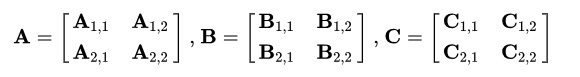
\includegraphics[width=10cm,keepaspectratio]{st1}
\end{frame}

\begin{frame}{행렬의 곱셈 : Strassen's Algorithm} 
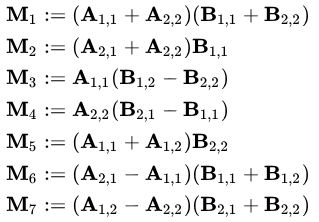
\includegraphics[width=10cm,keepaspectratio]{st2}

\end{frame}

\begin{frame}{행렬의 곱셈 : Strassen's Algorithm} 
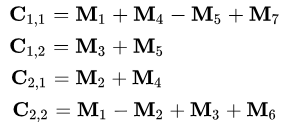
\includegraphics[width=10cm,keepaspectratio]{st3}

\end{frame}



\begin{frame}{행렬의 연산 : trace, transpose} 
\begin{itemize} 
\item trace : $tr(A) = \sum_i A_ii$
\item transpose : $(A^{T})_{ij} = A_ji$
\end{itemize}
\end{frame}

\begin{frame}{행렬의 연산 : determinant} 
행렬식은 재귀적으로 정의되며, 정사각행렬에서만 정의된다. 행렬 A의 행렬식 $det(A)$는 
\begin{itemize} 
\item 행렬의 size가 (1,1) : $A_{11}$
\item 행렬의 size가 (n,n) : $\sum^{n}_{i=1}(-1)^n det(minor(A, 1, i))$
여기서, $minor(A, i, j)$는 i번째 row와 j번째 column을 제거한 행렬을 말한다. 
\end{itemize}
\end{frame}


% \subsection{row space/column space} 

% \begin{frame}{row space} 
% \begin{itemize} 
% \item 
% \end{itemize}
% \end{frame}




% \subsection{선형변환과의 관계} 

% \begin{frame}{선형변환} 
% \begin{itemize} 
% \item 
% \end{itemize}
% \end{frame}

% \begin{frame}{선형변환과 행렬} 
% \begin{itemize} 
% \item 
% \end{itemize}
% \end{frame}

% \begin{frame}{행렬 곱과 함성함수 } 
% \begin{itemize} 
% \item 
% \end{itemize}
% \end{frame}

% \begin{frame}{역행렬과 역함수} 
% \begin{itemize} 
% \item 
% \end{itemize}
% \end{frame}


% \subsection{행렬의 변형} 

% \begin{frame}{Echelon Form} 
% \begin{itemize} 
% \item 
% \end{itemize}
% \end{frame}

% \begin{frame}{가우스 소거법} 
% \begin{itemize} 
% \item 
% \end{itemize}
% \end{frame}

% \begin{frame}{선형방정식 solver} 
% \begin{itemize} 
% \item 
% \end{itemize}
% \end{frame}


\end{document}


